\paragraph{Sats 7.13} $\bm{v}_{1},\ldots,\bm{v}_{r}$ vektorer i $\mathbb{R}^{n}$ 
och låt $A=\begin{pmatrix}\bm{v}_{1}&\ldots&\bm{v}_{r}\end{pmatrix}$.
Vektorerna $\bm{v}_{1},\ldots,\bm{v}_{r}$ utgör en bas för $\mathbb{R}^{n} \Leftrightarrow A\bm{x}=\bm{b}$ 
har en unik lösning för varje $\bm{b}\in\mathbb{R}^{n}$.

\paragraph{Sats 7.14} $\bm{v}_{1},\ldots,\bm{v}_{r}$ vektorer i $\mathbb{R}^{n}$.
Vektorerna $\bm{v}_{1},\ldots,\bm{v}_{r}$ utgör en bas $\Leftrightarrow r=n$ och $\bm{v}_{1},\ldots,\bm{v}_{r}$ är linjärt oberoende.

\paragraph{Definition} En mängd vektorer $V$ sägs ha dimension $h$ om varje bas för $V$ innehåller $n$ vektorer.

\paragraph{Sats 7.16} Låt $A$ vara en $n\times n$-matris.
Följande påståenden är ekvivalenta:
\begin{enumerate}
    \item $A\bm{x}=\bm{b}$ har en unik lösning för varje $\bm{b}\in\mathbb{R}^{n}$
    \item Varje reduktion av $A$ till en trappstegsmatris saknar vi fria kolumner
    \item Det går att reducera $A$ till identitetsmatrisen
    \item $A$ är inverterbar
    \item $det(A)\neq 0$
    \item kolumnerna i $A$ utgör en bas för $\mathbb{R}^{n}$
    \item $det(A^{t})=0$
    \item raderna i $A$ utgör en bas för $\mathbb{R}^{n}$
\end{enumerate}

\section{Baser i $\mathbb{R}^{n}$ (Avs 7.2)}
Vi ska nu skriva vektorer med koordinater i olika baser.
Vi är i $\mathbb{R}^{n}$. Låt $\bm{e}_{1},\ldots,\bm{e}_{n}$ vara standardbasen.
Antag att $\bm{f}_{1},\ldots,\bm{f}_{n}$ är ytterligare en bas.
En vektor $\bm{x}\in\mathbb{R}^{n}$ går att skriva
\begin{equation*}
    \bm{x}=x_{1}\bm{f}_{1}+\ldots+x_{n}\bm{f}_{n}=
    \underbrace{\begin{pmatrix}\bm{f}_{1}&\ldots&\bm{f}_{n}\end{pmatrix}}_{\text{Låt detta vara } F}
    \underbrace{\begin{pmatrix}x_{1}\\\vdots\\x_{n}\end{pmatrix}}_{=\bm{x_{f}}}
\end{equation*}
Alltså: $\bm{x}=F\bm{x}_{f}$\\
Vad är koordinaterna i basen $\bm{f}_1,\ldots,\bm{f}_n$?\\
Jo: $\bm{x}_F=F^{-1}\bm{x}$

\paragraph{Ex} Låt $\bm{v}=\begin{pmatrix}1\\2\\0\end{pmatrix}$ (i standardbasen).
Skriv koordinaterna för $\bm{v}$ i basen
\begin{equation*}
    \bm{f}_1=\begin{pmatrix}1\\2\\1\end{pmatrix}\text{, }
    \bm{f}_2=\begin{pmatrix}1\\1\\1\end{pmatrix}\text{ och }
    \bm{f}_3=\begin{pmatrix}0\\1\\2\end{pmatrix}
\end{equation*}
\subparagraph{Lösning} Kontrollera att $\bm{f}_1, \bm{f}_2, \bm{f}_3$ är en bas:
\begin{equation*}
    det\begin{pmatrix}1&1&0\\2&1&1\\1&0&2\end{pmatrix}=
    1\cdot\begin{vmatrix}1&1\\0&2\end{vmatrix}-1\cdot\begin{vmatrix}2&1\\1&2\end{vmatrix}=
    1\cdot (1\cdot 2-1\cdot 0)=1\cdot (2\cdot 2 - 1\cdot 1)=
    2-3=1\neq 0
\end{equation*}
$det\neq 0\Leftrightarrow$ Kolumnerna utgör en bas.\\
Vi vill hitta $x_1,x_2,$ och $x_3$ så att $f\begin{pmatrix}x_1\\x_2\\x_3\end{pmatrix}=\begin{pmatrix}1\\2\\0\end{pmatrix}$
där $F=\begin{pmatrix}\bm{f}_1&\bm{f}_2&\bm{f}_3\end{pmatrix}$.\\
Vi löser detta ekvationssystem:
\begin{equation*}
    \begin{pmatrix}
        1&1&0&1\\
        2&1&1&2\\
        1&0&2&0
    \end{pmatrix}
    \thicksim
    \begin{pmatrix}
        1&1&0&1\\
        0&-1&1&0\\
        0&-1&2&-1
    \end{pmatrix}
    \thicksim
    \begin{pmatrix}
        1&1&0&1\\
        0&1&-1&0\\
        0&0&1&-1
    \end{pmatrix}
    \thicksim
    \begin{pmatrix}
        1&1&0&1\\
        0&1&0&-1\\
        0&0&1&-1
    \end{pmatrix}
    \thicksim
    \begin{pmatrix}
        1&0&0&2\\
        0&1&0&-1\\
        0&0&1&-1
    \end{pmatrix}
    \Leftrightarrow
    \begin{cases}
        x_1=2\\
        x_2=-1\\
        x_3=-1
    \end{cases}
\end{equation*}
Alltså: $\bm{v}_F=\begin{pmatrix}2\\-1\\-1\end{pmatrix}$.\\
Kontroll: $2\bm{f}_1-1\bm{f}_2-1\bm{f}_3=\begin{pmatrix}1\\2\\0\end{pmatrix}$

\paragraph{7.19} Antag att $\begin{matrix}
    F=\begin{pmatrix}\bm{f}_1&\bm{f}_2&\ldots&\bm{f}_n\end{pmatrix}\\
    G=\begin{pmatrix}\bm{g}_1&\bm{g}_2&\ldots&\bm{g}_n\end{pmatrix}
\end{matrix}$ där $\bm{f}_1,\ldots,\bm{f}_2$ och $\bm{g}_1,\ldots,\bm{g}_2$ är baser för $\mathbb{R}^{n}$.
Då gäller att
\begin{itemize}
    \item $G\bm{x}_G=F\bm{x}_F$
    \item $\bm{x}_G=G^{-1}F\bm{x}_F$
    \item $\bm{x}_F=F^{-1}G\bm{x}_G$
\end{itemize}

\section{Linjära avbildningar och basbyten (Avs 7.3)}
Hur ser matrisen ut för en linjär avbildning om vi väljer andra baser än standardbasen?

\paragraph{Sats 7.22} Låt $\begin{matrix}
    G=\begin{pmatrix}\bm{g}_1&\ldots&\bm{g}_m\end{pmatrix}\text{ där }\bm{g}_1,\ldots,\bm{g}_m \text{ är en bas}\\
    H=\begin{pmatrix}\bm{h}_1&\ldots&\bm{h}_m\end{pmatrix}\text{ där }\bm{h}_1,\ldots,\bm{h}_m \text{ är en bas}
\end{matrix}$
Antag att $f:\mathbb{R}^n\rightarrow\mathbb{R}^m$ är en linjär avbildning.
Då är matrisen till $f$ relativt baserna $G$ och $H$ av
\begin{equation*}
    A_{H\rightarrow G}=
    \begin{pmatrix}
        f(\bm{h}_1)_G&f(\bm{h}_2)_G&\ldots&f(\bm{h}_n)_G
    \end{pmatrix}
\end{equation*}
Ett specialfall av satsen ges av att $m=n$ och $G=H$.
Det vill säga att vi har en linjär avbildning $F:\mathbb{R}^n\rightarrow\mathbb{R}^n$ och vi vill uttrycka den i basen $H$.

\paragraph{Sats 7.25} Om $G=\begin{pmatrix}\bm{g}_1&\ldots&\bm{g}_n\end{pmatrix}$ där $\bm{g}_1,\ldots,\bm{g}_n$ är en bas
och $f:\mathbb{R}^n\rightarrow\mathbb{R}^n$ är en linjär avbildning.
Då är matrisen till relativt $G$ given av $A_G=G^{-1}A_EG$ där $A_E$ är matrsien relativt standardbasen.

\clearpage
\paragraph{Ex} Skriv ner matrisen för projektion i $y=x$ i basen $\bm{g}_1=\begin{pmatrix}2\\1\end{pmatrix},\bm{g}_2=\begin{pmatrix}1\\1\end{pmatrix}$.
\subparagraph{Lösning} $\bm{g}_1,\bm{g}_2$ är en bas ty 
$det\begin{pmatrix}\bm{g}_1&\bm{g}_2\end{pmatrix}=det\begin{pmatrix}2&1\\1&1\end{pmatrix}=1$.
Vad är matrisen för projektionen i standardbasen?
Låt $P$ vara projektionen.
\begin{wrapfigure}{r}{0.46\textwidth}
    \centering
    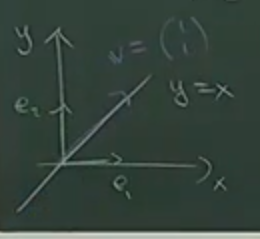
\includegraphics[scale=0.8]{imgs/img01.png}
\end{wrapfigure}
Då är matrisen 
\begin{equation*}
    A_E=\begin{pmatrix}P(\bm{e}_1)&P(\bm{e}_2)\end{pmatrix}=\frac{1}{2}\begin{pmatrix}1&1\\1&1\end{pmatrix}
\end{equation*}
\begin{equation*}
    P(\bm{e}_1)=\frac{\bm{e}_1\cdot \bm{v}}{\bm{v}\cdot \bm{v}}\cdot\bm{v}=\frac{(1,0)\cdot (1,1)}{(1,1)\cdot (1,1)}=\frac{1}{2}\begin{pmatrix}1\\1\end{pmatrix}
\end{equation*}
\begin{equation*}
    P(\bm{e}_2)=P(\bm{e}_1)
\end{equation*}
\begin{equation*}
    G=\begin{pmatrix}\bm{g}_1 & \bm{g}_2\end{pmatrix}=\begin{pmatrix}2&1\\1&1\end{pmatrix}
\end{equation*}
\begin{equation*}
    G^{-1}=\frac{1}{det(G)}\begin{pmatrix}1&-1\\-1&2\end{pmatrix}=\begin{pmatrix}1&-1\\-1&2\end{pmatrix}
\end{equation*}
\begin{equation*}
    A_G=G^{-1}A_EG=
    \frac{1}{2}\begin{pmatrix}1&-1\\-1&2\end{pmatrix}\begin{pmatrix}1&1\\1&1\end{pmatrix}\begin{pmatrix}2&1\\1&1\end{pmatrix}=
    \frac{1}{2}\begin{pmatrix}1&-1\\-1&2\end{pmatrix}\begin{pmatrix}3&2\\3&2\end{pmatrix}=
    \frac{1}{2}\begin{pmatrix}0&0\\3&2\end{pmatrix}
\end{equation*}

\section{ON-matriser och ON-baser (Avs 7.4)}
\paragraph{Definition} En bas sägs vara en \underline{ON-bas} om basvektorerna är ortogonala och av längd 1.

\paragraph{Definition} En linjär avbildning $f:\mathbb{R}^n\rightarrow\mathbb{R}^n$ kallas för en \underline{isometri} om
\begin{equation*}
    ||f(\bm{x})|| = ||\bm{x}||\text{ för alla }\bm{x}\in\mathbb{R}^n
\end{equation*}

\paragraph{Proposition 7.34} Om $f:\mathbb{R}^n\rightarrow\mathbb{R}^n$ är en isometri då $f(\bm{x})\cdot f(\bm{y})=\bm{x}\cdot\bm{y}$ för alla $\bm{x},\bm{y}\in\mathbb{R}^n$.
Alltså bevara isometrier vinklar mellan vektorer!

\paragraph{Definition} Om $f:\mathbb{R}^n\rightarrow\mathbb{R}^n$ är en isometri då kallas matrisen $f$ för en  ON-matris.

\paragraph{Sats 7.35} $A$ är en  ON-matris $\Leftrightarrow$ Kolumnerna i $A$ utgör en ON-bas.

\paragraph{Ex} $A=\begin{pmatrix}
    \frac{1}{\sqrt{3}}&\frac{1}{\sqrt{6}}&\frac{1}{\sqrt{2}}\\
    \frac{1}{\sqrt{3}}&\frac{1}{\sqrt{6}}&-\frac{1}{\sqrt{2}}\\
    \frac{1}{\sqrt{3}}&-\frac{2}{\sqrt{6}}&0
\end{pmatrix}$.
Vi kan kontrollera att kolumnerna i $A$ är parvis ortogonala och av längd $l$.
Alltså är kolumnerna en ON-bas.
Det betyder att $A$ är en isometri!

\paragraph{Sats 7.37} $A$ är en ON-matris $\Leftrightarrow A^{-1}=A^{t}$.

\paragraph{Ex} Inversen till $A$ ovan är $A^{-1}=\begin{pmatrix}
    \frac{1}{\sqrt{3}}&\frac{1}{\sqrt{3}}&\frac{1}{\sqrt{3}}\\
    \frac{1}{\sqrt{6}}&\frac{1}{\sqrt{6}}&-\frac{2}{\sqrt{6}}\\
    \frac{1}{\sqrt{2}}&-\frac{1}{\sqrt{2}}&0
\end{pmatrix}$.

\chapter{Egenvektorer och egenvärden}
\paragraph{Definition} Låt $A$ vara en $n\times n$-matris.
En vektor $\bm{v}\in\mathbb{R}^n,\bm{v}\neq\bm{0}$, kallas för en \underline{egenvektor till $A$} om det finns ett tal $\lambda$ så att $A\lambda=\lambda\bm{v}$.
Talet $\lambda$ kallas för \underline{egenvärdet till egenvektorn $\bm{v}$}.

\paragraph{Ex} LÅt $A$ vara $I_n$.
Varje vektor är en egenvektor med egenvärde 1.
Varför?
Jo för att för alla $\bm{v}$ gäller att $A\bm{v}=I_n\bm{v}=\bm{v}=1\cdot\bm{v}$

\paragraph{Ex} Låt $A$ vara en diagonal matris $A=
\begin{pmatrix}
    \lambda_1&0&\ldots&0\\
    0&\lambda_2&\ldots&0\\
    \vdots&\vdots&\ddots&\vdots\\
    0&0&\ldots&0&\lambda_n
\end{pmatrix}$.\\
Då är $\bm{e}_k$ en egenvektor med egenvärde $\lambda_k$.\\
Varför?
Jo $\begin{pmatrix}
    \lambda_1&&\\
    &\ddots&\\
    &&\lambda_n
\end{pmatrix}
\begin{pmatrix}
    0\\\vdots\\1\\\vdots\\0
\end{pmatrix}=
\lambda_k\begin{pmatrix}
    0\\\vdots\\1\\\vdots\\0
\end{pmatrix}=
\lambda_k\bm{e}_k$